\documentclass[12pt]{article}
 
\usepackage[margin=1in]{geometry} 
\usepackage{amsmath,amsthm,amssymb}
\usepackage{float}
\usepackage{tikz}
\usetikzlibrary{arrows,shapes,trees} % loads some tikz extensions
 
\begin{document}
 
\title{Homework 4}
\author{Josh Klontz
CSE 802}
 
\maketitle

\begin{enumerate}
\item \textbf{Consider the following data drawn from two distributions in two dimensions.}
\begin{enumerate}
\item \textbf{Compute the sample means.}
\begin{equation}
\begin{split}
m_1& = (-3.6, -1.2) \\
m_2& = (2.6, 0.4)
\end{split}
\end{equation}
\item \textbf{Compute the within-class scatter matrix.}
\begin{figure}[H]
\begin{verbatim}
function [ Si ] = scatter(x)
    mi = mean(x);
    Si = zeros(length(mi), length(mi));
    for i=1:length(x),
        Si = Si + transpose(x(i,:)-mi) * (x(i,:) - mi);
    end
end
\end{verbatim}
\caption{MATLAB code to compute a scatter matrix.}
\end{figure}
\begin{equation}
S_w = \left[ \begin{array}{cc} 70.4 & 10.2 \\ 10.2 & 56 \end{array} \right]
\end{equation}
\item \textbf{Compute the between-class scatter matrix.}
\begin{equation}
S_b = \left[ \begin{array}{cc} 38.44 & 9.92 \\ 9.92 & 2.56 \end{array} \right]
\end{equation}
\item \textbf{Find the Fisher Linear Discriminant for this data.}
\begin{equation}
\text{Fisher Linear Discriminant} = (-0.0862, -0.0129)
\end{equation}
\item \textbf{Plot the data points and the discriminant.}
\begin{figure}[H]
\centering
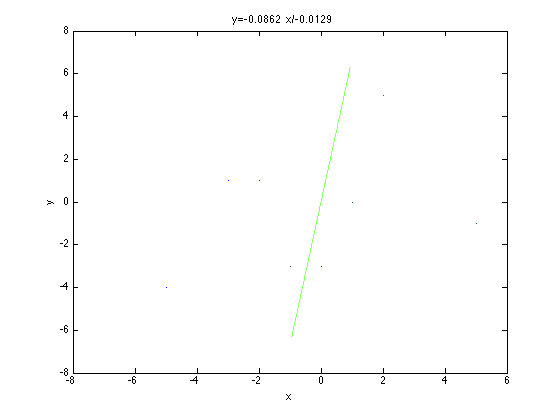
\includegraphics[width=4in]{1}
\caption{The points and the discriminant.}
\end{figure}
\end{enumerate}
\item \textbf{Face Recognition!}
\begin{enumerate}
\item \textbf{Align the face images based on the location of the
eyes and resize them.} \\
Completed using OpenBR: \texttt{br -algorithm RegisterFace -enroll FERET\_100 FERET\_100\_registered}
\item \textbf{Calculate the set of top 100 Eigenfaces and Fisherfaces; visualize
the top 20 basis faces to see what they look like.}
\begin{figure}[H]
\begin{verbatim}
function [m vecs vals] = pca(data)
    m = zeros(size(data,1),1);
    for i=1:size(data,1),
        m(i) = mean(data(i,:));
    end
    for i=1:size(data,2),
        data(:,i) = data(:,i)-m;
    end
    scatter = transpose(data)*data;
    [vecs vals] = eig(scatter);
    vecs = data * vecs;
end
\end{verbatim}
\caption{MATLAB code for PCA.}
\end{figure}
\end{enumerate}
\end{enumerate}
\end{document}
